%% Chapter WP Models

\section{Store}\label{sec-store}


The Store memory model is the default model for the \textsf{WP}
plug-in. Heap values are stored in a global array. Pointer values are
translated to an index of this array.\par

In order to generate reasonable proof obligations, the values stored
in the global array are not the machine-ones, but the logic
ones. Hence, all \textsf{C} integer types are represented by
mathematical integers.\par

A consequence is that heterogeneous cast of pointers can not be
translated with this model. For instance, you can not cast a pointer
to \whyinline{int} into a pointer to \whyinline{char}, and then access to
the internal representation of an \whyinline{int} value in memory. In the 
same flavor, the Store model does not support union. 


The Store model specifies the memory state by two arrays.
\begin{enumerate}
   \item A {\it store} (also called {\it memory}) represents the whole heap see
     figure~\ref{fig:mem}.  A store is an array of elementary cells
     (indexed by an address)
     containing encoded \whyinline{data}. 
     The \whyinline{data} are described in the 
     section~\ref{ssec-acsl-value}
   \item An {\it allocation table} informs about the validity 
     of the access to these cells.
\end{enumerate}


\subsection{C variable representation}

The Store model associates to each C variable $x$ a base of address
\whyinline{base(x)}. 
At the allocation of a variable $x$, the allocation table is updated 
such as it associates to \whyinline{base(x)} the number \whyinline{n} 
of cells corresponding to the type of $x$ (see figure~\ref{fig:sz_base} 
and~\ref{fig:sz_compl}). The number $0$ denotes unallocated variables.
Then, the encoded value of $x$ is stored to a block of the {\it memory} 
corresponding to the \whyinline{n} first cells starting from the index
\whyinline{addr(base(x),0)}. \par

When using the \whyinline{-wp-logicvar} option, some C variables can be
viewed as logic variables. 
In such case, another representation (described in 
section~\ref{sec-funvar}) is used.\par


\begin{figure}[ht!]
\begin{center}
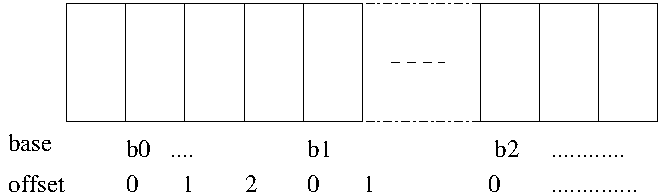
\includegraphics[height=4cm]{mem}
\end{center}
\caption{The {\it memory}}
\label{fig:mem}
\end{figure}


\subsection{Addresses}\label{ssec-store-addr}

The constructor for addresses is: 
\begin{description}
  \item{\whyinline{addr(b,ofs)}} returns an integer (which represent
an address). This integer is computed from a base
    \whyinline{b} and an offset \whyinline{ofs} (think about a binary
    applicative constructor)
\end{description} 

Two projections can be defined for such addresses: 
\begin{description}
  \item{\whyinline{base(x)}} returns the base of an address
    \whyinline{x} such that:\\  
    \whyinline{axiom base_addr: forall b,ofs:int. base(addr(b,ofs)) = b}
  \item{\whyinline{offset(x)}} returns the offset of an address
    \whyinline{x} such that:\\ 
    \whyinline{axiom offset_addr: forall b,ofs:int. offset(addr(b,ofs)) = ofs}
\end{description} 

An address can be shifted: 
\begin{description}
  \item \whyinline{addr_shift(a,ofs)} returns an address shifted of \whyinline{ofs} 
cells from the address \whyinline{a} such that \\ 
\whyinline{base (addr_shift(a,ofs)) = base(a)} and \\
\whyinline{offset (addr_shift(a,ofs)) = offset(a)+ofs}.
\end{description} 

An address \whyinline{a} has to be converted into a logic pointer
(see section~\ref{ssec-acsl-ptr}):\whyinline{pointer_of_addr(a)} and a logic
pointer \whyinline{p} can, also, be converted into an address:
\whyinline{addr_of_pointer(p)}.


\subsection{Blocks and zones}\label{ssec-store-addrg}

An address is too weak to specify the place into the heap where a
value is stored.  

\begin{figure}[ht!]
\begin{center}
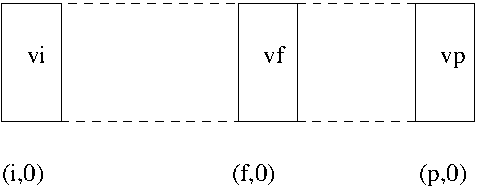
\includegraphics[height=4cm]{size_base}
\end{center}
\caption{Typed representation of objects}
\label{fig:sz_base}
\end{figure}

The address of base specifies the first cell where the value is stored, 
and a value is stored over a number of cells corresponding to the size of
this value (Think about some kind of C \whyinline{sizeof}, but more abstract.).
In the Store model, the size of values of basic types is $1$, 
this is the case of the integer \whyinline{i}, 
the float \whyinline{f} and the pointer \whyinline{p} in the 
figure~\ref{fig:sz_base}.
The size of a more complex value, such as an array and a record, is the 
number of objects of which it is comprised.
The figure~\ref{fig:sz_compl} considers the following code: 

\begin{ccode}
 struct S 
 { int f[2]; 
   float g;
 } ; 

 S s;
 
 S t[2];
\end{ccode}

\begin{figure}[ht!]
\begin{center}
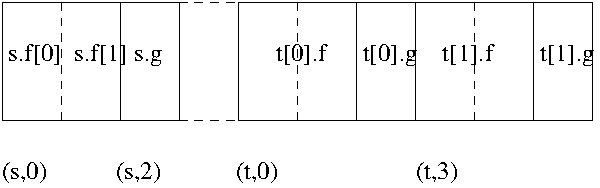
\includegraphics[height=4cm]{size_compl}
\end{center}
\caption{Typed representation of objects}
\label{fig:sz_compl}
\end{figure}



The representation of \whyinline{s} needs three cells in the {\it memory}, 
the representation of \whyinline{t} needs six cells, three for each 
element. 

\subsubsection{Blocks}\label{ssec-store-bloc}

The pair of an address and a
number of cells forms a block of {\it memory}.
The constructors of such bocks are:
\begin{description}
   \item{\whyinline{zempty}} is the empty block. Nothing can be stored 
     there. 
   \item{\whyinline{zrange(b,ofs,n)}} represents the {\it memory} block
     composed of the
     \whyinline{n} cells starting from the address \whyinline{addr(b,ofs)}. 
     This block can be used to load and store records and arrays in the 
     {\it memory}.
   \item \whyinline{zrange_of_addr(a)} returns the {\it memory} block
     composed of one cell for a basic type at the address \whyinline{a}.
     Its definition is: \\
     \whyinline{zrange_of_addr(a) = zrange(base(a),offset(a),1)}.
   \item \whyinline{zrange_of_addr_range(a,ofs,n)} returns the {\it memory}
     block of \whyinline{n} cells from the address \whyinline{a}
     shifted by \whyinline{ofs}.
     Its definition is: \\
     \whyinline{zrange_of_addr_range(a,ofs,n) = zrange(base(a),offset(a)+ofs,n)}.
\end{description}


Then, the validity of an address and the separation between two
addresses hang on the number of cells associated to the addresses:
\begin{description}
 \item{\whyinline{valid(ta,a,n)}} holds iff all \whyinline{n} cells
   from the address \whyinline{a} are included into the number of
   cells associated to the \whyinline{base(a)} into the allocation
   table \whyinline{ta}.
 \item{\whyinline{separated_on_addr(a,n,a',n')}} holds iff there is no
   overlap between the \whyinline{n} cells from \whyinline{a} and the
   \whyinline{n'} cells from \whyinline{a'}.
\end{description}


\subsubsection{Zones}\label{ssec-store-zone}

 The type \whyinline{zone} is defined as sets of 
 blocks. Blocks identify a number of adjacent cells related to an
 address of base, and zones allow the identification of any partition
 of the whole {\it memory}\/. \par

 In the logic language $\cal{L}$, block constructs are promoted to 
 singletons of type \whyinline{zone}.
 Just an union operator is necessary to build complex zones from zones
 and/or blocks. Zones can be compared using classical set operators:
 \begin{description}
   \item{\whyinline{zunion(z,z')}} unions of two {\it memory} zones.
   \item{\whyinline{included(z,z')}} holds if the {\it memory} zone
     \whyinline{z} is included in the {\it memory} zone \whyinline{z'}.
   \item{\whyinline{separated(z,z')}} holds if the {\it memory} zone \whyinline{z} does not
     intersect the {\it memory} zone \whyinline{z'}. This operation is used for
     the translation of \whyinline{\\separated} function of \textsf{ACSL}.
 \end{description}

 A zone equivalents to singleton is a particular zone since it defined a block which
 can content as well as basic data than complex data as arrays and records of $\cal{L}$.
 It is possible to recognize such zone: 
\begin{description}
   \item{\whyinline{is_bloc(z)}} holds if and only if it exists
   \whyinline{x, ofs>0, n>0} such that \whyinline{z = zrange(base(x),ofs,n)}.
\end{description}
 

 The validity of a location, the \textsf{ACSL} predicate
 \cinline{valid(l)} is translated as \whyinline{valid(ta,addr_of(l),n)} when
 \whyinline{n} is the number of cells of the location \whyinline{l}.

 The separation of two location, the \textsf{ACSL} predicate
 \cinline{separated(l,l')} is translated by 
 \whyinline{separated(zone_of(l),zone_of(l'))}


\subsection{Variable scope}

The allocation table informs about how many cells have
been allocated for each address of base. 
As said in section~\ref{ssec-store-addrg}, querying the
allocation table defines the validity of an address for a number of
cells. It can also informs about the scope of variables.  An unallocated
\whyinline{base(x)} is associated to $0$ cell into the allocation
table. \par

Moreover, we need a property over \whyinline{base(x)} parametrized
by a store and a allocation to hang on the bound of the C variable $x$
scope. Hence, the property \whyinline{is_fresh(m,ta,b)} means that all
addresses such as their base is \whyinline{b}, cannot be loaded into the
store \whyinline{m} and cannot be valid into \whyinline{ta}. \par


During a WP computation, the scope of different kinds of variables 
is specified as follows:
\begin{description}
  \item Global variables are marked as they are already allocated into 
the initial allocation table, 
 \item Formal parameters are specified as they were out of the scope
   of the initial memory configuration. Their scopes are open before
   the precondition,
  \item The local variables scopes are open after the precondition and are
  closed before the post-condition.
\end{description}

Lets consider the following piece of code:
\begin{ccode}

int X;

/*@ requires \valid(p);
    assigns *p;
    ensures  *p == X;
*/
void f (int *p)
{
 int * q; 
 q=p;
 *q = X;

}

\end{ccode}


 Running the WP computation with the Store model we get the 
following environment : 
\begin{whycode}
Global 'X'
wp_store_ex.c:1: int X ;
function X_X () : int = 2

Local 'p'
wp_store_ex.c:7: int* p ;
function X_p () : int = 1

Local 'q'
wp_store_ex.c:9: int* q ;
function X_q () : int = 3

Global 'X'
wp_store_ex.c:1: Global allocation table
axiom Alloc_X: forall ta:int farray.
     global(ta)
  -> (ta[X_X] = 1)
\end{whycode}

 For each C variable, a base is defined \whyinline{X_X,X_p,X_q}.  The
 axiom \whyinline{Alloc_x} specifies the global scope of the variable
 \whyinline{X}. If we get the scope mark \whyinline{global(ta)} then 
 \whyinline{X} is valid in \whyinline{ta} and the size associated is 
 \whyinline{1}.  
  

 The WP computation for the post-condition produces the formula:

 \begin{whycode}
 forall m_0:data farray.
  forall ta_0:int farray.
     global(ta_0) 
  -> (ta_0[X_p] = 0)
  -> is_fresh(m_0, ta_0, X_p)
  -> (let ta_0= ta_0[X_p->1] in
         valid(ta_0, {m_0[addr(X_p,0)]}, 1)
      -> (ta_0[X_q] = 0)
      -> is_fresh(m_0, ta_0, X_q)
      -> (let ta_0= ta_0[X_q->1] in
          let m_1= m_0[addr(X_q,0)->{{m_0[addr(X_p,0)]}}] in
          let m_2= m_1[{m_1[addr(X_q,0)]}->{{m_1[addr(X_X,0)]}}] in
          let ta_0= ta_0[X_q->0] in
             is_fresh(m_2, ta_0, X_q)
          -> (let ta_0= ta_0[X_p->0] in
                 is_fresh(m_2, ta_0, X_p)
              -> ({m_2[{m_0[addr(X_p,0)]}]} = {m_2[addr(X_X,0)]})))) 
 \end{whycode}

First, the {\it memory} and the allocation table are introduced. 
The first hypothesis, \whyinline{global(ta_0)},
triggers the axiom \whyinline{Alloc_X} and we have \whyinline{X}
already allocated in the initial allocation table. 

The two next hypotheses: 
  \begin{whycode}
 (ta_0[X_p] = 0)
  -> is_fresh(m_0, ta_0, X_p) 
 \end{whycode}

say that the formal parameter \whyinline{p} is out of the scope of the
initial memory configuration: its base of address is not valid in the 
allocation table and it cannot been loaded in the initial memory.

As formal parameters are in the scope of the precondition, 
the allocation table has to be updated before the precondition computation.
After the precondition translation, the two hypotheses
 
\begin{whycode}
  (ta_0[X_q] = 0)
  -> is_fresh(m_0, ta_0, X_q)
\end{whycode}
 
state that the local variable \whyinline{q} is out of the scope of
the precondition and then the allocation table is updated before
formulating the body of the function.
Before asserting the post-condition, the scope of the local variable 
is closed: the allocation table is updated and its address cannot be 
loaded in the final memory. On the contrary, the scope of the formal
parameter is still open, since the formal parameters are in the scope 
of the post-condition. 

\subsection{The store operations}
  
 The store is an array of \whyinline{data} indexed by addresses
 (see figure~\ref{fig:mem} and section~\ref{ssec-acsl-rec} 
 for the logic records).


\subsubsection{Data}\label{ssec-acsl-value}

 The store is specified into logic array of
 \whyinline{data}, indexed by addresses. The type \whyinline{data} is a
 common type representation for all types of values supported by the
 \textsf{ACSL}. That means a field of type $\tau$ contains an object
 of type \whyinline{data} in the representation of the
 record. However, the value of a field of type $\tau$ must be
 specified by an object of type $\tau$. 




 \subsubsection{Loading and assignment of basic objects}
   As basic type object only needs one cell to be stored in the Store
   model, loading/writing a value of a basic type are translated in
   simple access/update from the store, but this value has to be
   encoded/decoded as defined in section~\ref{ssec-acsl-rec}. The format
   for integers and floats are thus defined in section~\ref{ssec-acsl-rec},
   for store address, we specify the special format
   \whyinline{addr_format}.
   
   
 \subsubsection{Loading and assignment of records and arrays}
 
   In the Store model, it is possible to load or assign records or
   arrays using the combination of two steps. 

   First, loading and assignment of a block of \whyinline{data} in
   the memory:
   \begin{description}
    \item{\whyinline{access_range(m,z)}} loads in one time a zone
       \whyinline{z} in the memory \whyinline{m} and returns a
      \whyinline{data}. Note that \whyinline{z} has to be 
      \whyinline{zrange(b,ofs,n)} with \whyinline{n >0} to make sense. 
      This is what ensured the predicate \whyinline{is_block(z)}.
      
      \item{\whyinline{update_range(m,z,v)}} updates in one operation
        the zone \whyinline{z} by the \whyinline{data} \whyinline{v}
        in the memory \whyinline{m}, with \whyinline{is_block(z)}.
   \end{description}

   Secondly, decoding/encoding the data (involved in the first step)
   with the format of the type of the object. 

   The two following example illustrate this mechanism.

   Suppose this simple function:

   \begin{ccode}
   int t[4]; 
   /*@ assigns t[1]; 
    ensures t == {\old(t) \with [1] = (int)3}; 
   */

  void modif_array(void)
  { t[1] =3;}

   \end{ccode}

  
   The generated output in $\cal{L}$ defines, at first, how to update
   and access to indexed values of the array of $4$ int: 

   \begin{whycode}

axiom Loaded_int_4_idx:
  forall m:data farray.
  forall p:int.
  forall i:int.
     (0 <= i)
  -> (i < 4)
  -> (decode(Afmt_int_4,access_range(m,zrange_of_addr_range(p,0,4)))[i]
      = decode(int_format,m[addr_shift(p,i)]))
axiom Updated_int_4:
 forall m:data farray.
 forall i:int.
 forall e:int.
 forall p:int.
    (0 <= i)
 -> (i < 4)
 -> Eqarr_int_4(
     decode(Afmt_int_4,
        access_range(m[addr_shift(p,i)<-encode(int_format,e)],
          zrange_of_addr_range(p,0,4))),
     decode(Afmt_int_4,access_range(m,zrange_of_addr_range(p,0,4)))[i<-e])
 \end{whycode}
   

Notice that the update definition requires the equality of array of
$4$ int (definition \whyinline{Eqarr_int_4}) defined in the
\textsf{ACSL} model see section~\ref{ssec-acsl-eq}. \par 


In the Store model, the access to the whole array \whyinline{t} is the
 \whyinline{data} loaded from a block of the store \whyinline{m},
 starting from the address \whyinline{(p,0)} over $4$ cells :
\whyinline {access_range(m,zrange_of_addr_range(p,0,4))}. This
\whyinline{data} is decoded as an array of $4$ int. The axiom
\whyinline{Loaded_int_4_idx} expresses that accessing to the $i^{nth}$
index of this array is the same that accessing to the address of the
beginning of the array \whyinline{p} shifted by $i$ times the size of
\whyinline{int} (i.e. $1$ since int is a basic type).
The update operation is defined in the same flavor. \par 


The postcondition is formulated as: 
\begin{whycode}
goal store_full_modif_array_post_1:
  forall m:data farray.
  Eqarr_int_4(
    decode(Afmt_int_4,
      access_range(m[addr(X_t,1)<-encode(int_format,3)],zrange(X_t,0,4))),
    decode(Afmt_int_4,access_range(m,zrange(X_t,0,4)))[1
      <-as_int(sint32_format,3)])
\end{whycode}
 Informally, it is to say that the array \whyinline{t} loaded in the memory
 after having updated the cell at the address \whyinline{addr(X_t,1)}
 with the \whyinline{data} encoding of the int \whyinline{3} is equal
 to the updated array loaded in the memory
 \whyinline{decode(Afmt_int_4,access_range(m,zrange(X_t,0,4)))} at
 index \whyinline{1} with the \whyinline{data} encoding of the int
 \whyinline{3}.\par

 \whyinline{Afmt_int_4} is the format of array of $4$ int for the Store
  model. The model Store generated its own format for each array
  and record type. \par



 In the case of a record, the same kind of definitions occurs but this
 time, instead of generalize over all bound indexed (\whyinline{0 <= i} 
 and \whyinline{i < 4}) an axiom for loading and another for
 storing are defined for each field of the record. \par

  
\subsection{The assigns clause specification}

  The WP computation needs two different specifications of an assigns
  clause:
\subsubsection{Assigns as a memory operation} 
 The memory operation \whyinline{update_havoc(m,z,v)} returns a memory
 where all addresses contains in the zone \whyinline{z} contains a
 \whyinline{data}.  This function is quite similar than
 \whyinline{update_range} at first glance. In fact, they are
 different, \whyinline{z} can be any zone and the stored
 \whyinline{x} is never encoded or decoded.

\subsubsection{Assigns as a property between two memory states}

 In the Store model there are two different ways to express the assigns clause
 as a goal: 
 \begin{description}
    \item{Relational:} the predicate
      \whyinline{is_havoc(ta_init,m_init,z,ta_fin,m_fin)} holds if
      from the memory configuration \whyinline{(ta_init,m_init)} to
      \whyinline{(ta_fin,m_fin)} excluded all addresses in the zone
      \whyinline{z} nothing has changed.
      
%    \item{Zone inclusions:} TODO Lo�c... \whyinline{included(z_c,z_a)}
 \end{description}
 


